\documentclass[a4paper, 14pt]{article}
\usepackage[utf8]{inputenc}
\usepackage{graphicx}
\usepackage{float}%"Плавающие" картинки
\usepackage{wrapfig}%Обтекание фигур (таблиц, картинок и прочего)
\usepackage{amsmath, amssymb, mathtext, amsthm}
\usepackage[T1, T2A]{fontenc}
\usepackage[english, russian]{babel}
\usepackage[left=2cm,right=2cm, top=2cm, bottom=2cm]{geometry}
\begin{titlepage}
\begin{center}

\hfill \break

\large{Министерство науки и высшего образования Российской~Федерации}\\
\footnotesize{Федеральное государственное автономное образовательное учреждение высшего образования}\\ 
\small{\textbf{«КАЗАНСКИЙ (ПРИВОЛЖСКИЙ) ФЕДЕРАЛЬНЫЙ УНИВЕРСИТЕТ»}}\\

\hfill \break
\normalsize{Институт механики и математики им. Н. И. Лобачевского}\\

\hfill \break
\normalsize{Направление подготовки: 01.01.03 Механика и математическое моделирование}\\

\vspace{25mm}
\large{Курсовая работа}\\
\end{center}

\vspace{20mm}
\noindent
Студентка 3 курса \\
группы 05-001 \\
<<\underline{\hspace{0,75cm}}>> \underline{\hspace{2cm}}\the\year~г.

\hfill \break
Научный руководитель \\
<<\underline{\hspace{0,75cm}}>>\underline{\hspace{2cm}}\the\year~г.

\vspace{\fill}

\begin{center}
    Казань, \the\year
\end{center}
\thispagestyle{empty}

\end{titlepage}

\begin{document}
\newpage
\tableofcontents
\newpage
\section{Введение}
\subsection{Актуальность работы}
Кровь—это соеденительная ткань внутри организма, она состоит из форменных элементов (эритроцитов, лейкоцитов, тромбоцитов), а так же водного раствора белков и свёртывающих веществ-плазмы. Объёмная доля форменных элементов в общем объеме называется гематокритом и составляет примерно 45\%
\begin{figure}[h]
\centering
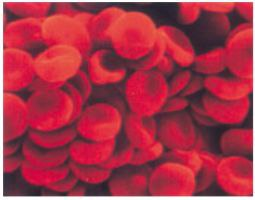
\includegraphics[width=0.3\linewidth]{erotr.jpg}
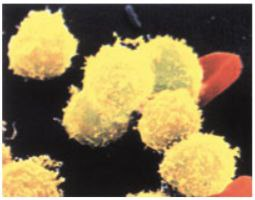
\includegraphics[width=0.3\linewidth]{leiko.jpg}
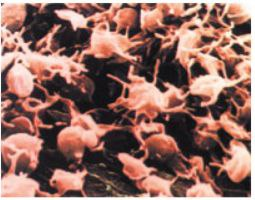
\includegraphics[width=0.3\linewidth]{trombo.jpg}
\caption{ Электронные фотографии элементов крови.1—эритроциты, 2—лейкоциты, 3—тромбоциты. \cite{rls:2003}}
\label{fig:mpr}
\end{figure}\\

Функций у крови несколько: она является транспортным средством, поддерживает постоянство «внутренней среды» организма (гомеостаз), играет главную роль в защите от чужеродных веществ.

С развитием медицины и науки в целом, появилась необходимость в изучении течения крови. Зная как движется кровь в организме, мы получаем более масштабную картину того, как работает наш организм, можем помочь поставить диагноз, спрогнозировать развитие заболеваний, подобрать оптимально лечение.

В изучении течения крови не малую роль играет вычислительная гидродинамика. Её главное достоинство— возможность проводить практически неограниченное число численных экспериментов без опасности для жизни и здоровья испытуемого, в отличие от традиционных методов лечения, где все эксперименты ставятся на органах животных.

\subsection{Общее описание течения крови в организме}
Кровь движется по замкнутой системе сосудов,циркулируя от сердца и обратно. Кровеносная система человека — сложная, разветвленная сеть, состоящая из вен, артерий и капилляров, соединяющих артерии и вены. Кровообращение состоит из двух кругов.

Малый круг начинается в правом желудочке, при сокращении которого венозная кровь попадает в легочный ствол и, протекая через легкие, отдает диоксид углерода и насыщается кислородом. Обогащенная кислородом кровь из легких по легочным венам поступает в левое предсердие, где заканчивается малый круг. Большой круг начинается в левом желудочке, при сокращении которого кровь, обогащенная кислородом, нагнетается в аорту, артерии, артериолы и капилляры всех органов и тканей, а оттуда по венулам и венам притекает в правое предсердие, где и заканчивается большой круг.

Кровь движется по сосудам под воздействием периодических сокращений сердечной мышцы, описываемых сердечным циклом. Под сердечным циклом понимают период, охватывающий одно сокращение и одно расслабление предсердий и желудочков. Общая длительность сердечного цикла при частоте сердечных сокращений 75 уд/мин равна 0,8 с. Систола (0,33с) — фаза сердечного цикла, включающая сокращение миокарда и изгнание крови из сердца в сосудистую систему. Диастола (0,47) — фаза сердечного цикла, включающая расслабление миокарда и наполнение полостей сердца кровью.

Все сосуды в человеческом организме можно условно разделить на аорту(диаметр ~ 15.3 мм), артерии(диаметр ~ 0.5—2.5 мм), полые вены(диаметр ~ 12 мм), вены (диаметр ~ 0.75—2.7 мм) и капилляры(диаметр ~ 8 мкм).

Стенку кровеносного сосуда (за исключением капилляров) условно можно разделить на три слоя: интима – внутренний слой, медиа – средний слой, адвентиция – внешний слой (рис. 2).
В зависимости от состава сосудистой стенки, артерии условно делят на эластичный или мышечный типы . Артерии эластичного типа – сосуды относительно большого диаметра, расположенные ближе к сердцу (например аорта), медиа которых содержит большое количество упругих мембран. Число упругих мембран убывает при уменьшении размера сосуда. Они практически отсутствуют в артериях мышечного типа. Артерии мышечного типа находятся на периферии (например, бедренная артерия). В среднем слое артерий мышечного типа доминируют гладкомышечные клетки. Вены, в отличие от артерий, делятся по размеру внутреннего диаметра. У вен толщина стенок и толщина среднего слоя намного меньше, чем у артерий. При этом у вен толще внешний слой. [\cite{rhodin:1980}] 


\begin{figure}[h]
\centering
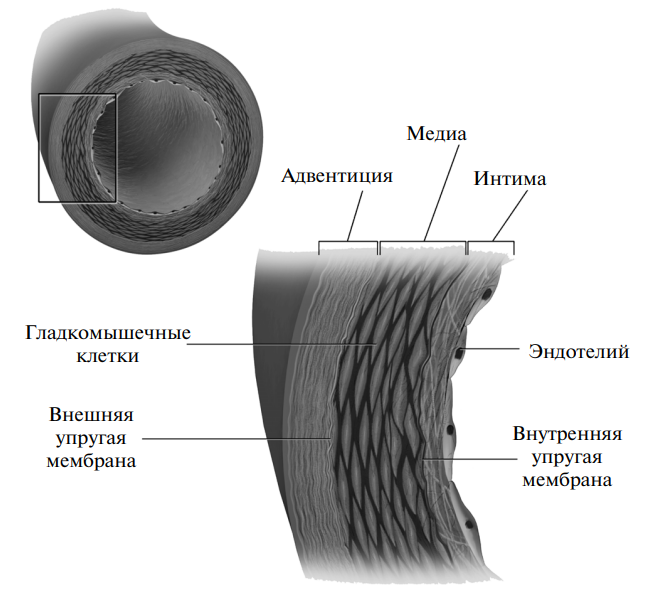
\includegraphics[width=0.3\linewidth]{stenki.png}
\caption{ Типовое строение стенки кровеносного сосуда \cite{blausen:2014}.}
\label{fig:mpr}
\end{figure}

Кровь, двигаясь по сосудам, испытывает сопротивление движению со стороны сосудов и из-за её вязкости. Величина сопротивления зависит от диаметра сосуда, его длины, скорости кровотока. Поэтому сердце выбрасывает кровь в сосудистую систему под большим давлением. В разных отделах сосудистой системы давление крови будет разным. В аорте среднее давление в 100 мм рт.ст. колеблется в диапазоне от 120 мм рт.ст. при систоле до 80 мм рт.ст. при диастоле. Разница между ними—пульсовое давление. По мере движения крови давление в сосудистом русле падает. Таким образом, непрерывные, ритмические сокращения сердца, преодолевая сопротивление, создают и поддерживают разность кровяного давления между артериальным и венозным участком сосудистой системы. Эта разность давлений и является главной причиной движения крови по сосудам из области высокого давления в область более низкого.

При движении крови по сосудам различают линейную и объемную скорость кровотока. Линейная скорость определяется суммарным сечением сосудистой системы. Она максимальна в аорте — до 50 см/сек и минимальна в капиллярах — около нуля. В венозном отделе сосудистой системы линейная скорость вновь возрастает. Линейная скорость в полых венах в два раза меньше, чем в аорте и равна примерно 25 см/мин, поскольку в организме на одну артерию приходится две вены,Объемная скорость кровотока — это количество крови, протекающее через общее сечение сосудистой системы в единицу времени. Она одинакова во всех отделах сосудистой системы. Через любое сечение сосудистой системы в единицу времени всегда проходит одинаковое количество крови.

Состоит кровь, как уже было сказано ранее, из форменных клеток и плазмы. Численную долю объёма крови, приходящуюся на клетки, называют гематокритом. Его значение варьируется в зависимости от пола, возраста в границах 0.37 - 0.54. 99 \% гематокрита приходится на эритроциты. Эритроциты— двояковогнутые диски, размерами 7-8 мкм, их количество так же зависит от параметров организма и варьируется от 3.8 до 5.6 миллионов клеток на 1 мкл, а объём от 73 до 83 $10^{-15}$л. Лейкоциты-ядерные клетки округлой формы, их количество на 1 мкл составляет 4.5–11 тысяч, а размеры 4-20 мкм, количество тромбоцитов 150-400 тысяч на 1 мкл и размеры 2-4 мкм. 60 \% от объёма крови приходится на плазму — жидкое межклеточное вещество, содержащее 90—93 \% воды и 7—10 \% сухого вещества (белки, углеводы, соли).

Вязкость крови обычно оценивают: 4.3-4.9 мПа$\cdot$с, а её плотность 1.052—1.0604 г/см\textsuperscript{3}. В зависимости от наличия заболеваний, определенного образа жизни и питания эти показатели могут отходить от нормы. 

Ламинарное течение – упорядоченный режим течения вязкой жидкости, характеризующийся отсутствием перемешивания между слоями жидкости. Течение жидкости с завихрениями называется турбулентным. 
Наличие условий, при которых ламинарное течение перестает быть устойчивым, зависит от числа Рейнольдса:
$$Re=\frac{V\cdot S\cdot \rho}{\eta}$$
где v – скорость течения жидкости, S– сечение трубы, $\rho$- плотность жидкости, $\eta$- вязкость жидкости.

Для гладких труб Re= 2300. Если Re известно, то становится возможным предсказать, будет ли поток ламинарным или турбулентным. Если для определенного течения число Рейнольдса не превышает некоторого критического значения, то ламинарное течение устойчиво. Если же оно больше, то в потоке жидкости возникают завихрения. Re для крови равно 900-1600. Движение крови в организме, в основном, ламинарное. Однако, при определенных условиях, кровоток может приобретать и турбулентный характер.

Турбулентность проявляется в полостях сердца (велико значение d), в аорте и вблизи клапанов сердца (высокая скорость движения крови). При интенсивной физической нагрузке скорость движения крови увеличивается, и это может вызвать турбулентность в кровотоке. При некоторых патологических процессах, приводящих к аномальному снижению вязкости крови, кровоток в крупных кровеносных сосудах может стать турбулентным.  При наличии атеросклеротических бляшек в просвете сосудов имеются локальные сужения, приводящие к возникновению турбулентности в течении крови. 

\subsection{Вывод}
 С точки зрения гидродинамики кровоток представляет из себя пульсирующее с низкой частотой течение мелкодисперсной суспензии в замкнутой системе каналов кругового сечения с эластичными стенками, осложнённое локальными эффектами ламинарно-турбулентного перехода.

\section{Подходы к моделированию кровотока}
\subsection{Детальное моделирование}
Моделировать кровь можно как жидкость со взвешенными в ней клетками крови, которые могут рассматриваться, как совокупность частиц и сил, действующих между ними. Эритроциты гораздо крупнее остальных клеток крови и они составляют большую часть её объёма, соответственно они и будут определять механичисткие свойства крови. Плазма крови — раствор крупных молекул, но при масштабах движения и при скоростях сдвига, обычно встречающихся в кровеносных сосудах, ее можно считать однородной ньютоновской жидкостью  и описывать уравнениями Новье-Стокса. То есть нам нужно учитывать взаимодействие частиц с жидкостью и друг с другом. Такую задачу удобно решать методом диссипативной динамики частиц.

Диссипативная динамика частиц—это метод, в котором каждая частица описывает небольшой объем моделируемой среды, а не отдельную молекулу. Их взаимодействие определяется консервативными $F^C_{ij}$ (не зависящими от 
траектории), диссипативными $F^D_{ij}$(силы, при действии которых полная механическая энергия  системы убывает, переходя в другие, не механические формы энергии) и случайными силами $F^R_{ij}$, действующими между двумя частицами:
$$\mathbf{F^C_{ij}}=F^C_{ij}(r_{ij})\mathbf{\hat{r_{ij}}}$$
$$\mathbf{F^D_{ij}}=-\gamma \omega^D(r_{ij}) (\mathbf{v_{ij}} \cdot \mathbf{\hat{r_{ij}}})\mathbf{\hat{r_{ij}}}$$
$$\mathbf{F^R_{ij}}=\sigma \omega^R(r_{ij}) \dfrac{\varepsilon_{ij}}{\sqrt{\bigtriangleup t}} \mathbf{\hat{r_{ij}}}$$\\
где $\mathbf{r_{i}}$— радиус-вектор i-ой частицы, $\mathbf{r_{ij}}=\mathbf{r_{j}} - \mathbf{r_{j}}$ ,
$r_{ij}=|\mathbf{r_{ij}}|$,
$\mathbf{\hat{r_{ij}}}=\mathbf{r_{ij}}/{r_{ij}}$,
$\mathbf{v_{ij}}=\mathbf{v_{j} - \mathbf{v_{j}}}$— разница между скоростями двух частиц, $\bigtriangleup t$—шаг по времени, $\gamma, \sigma$ — это  коэффициенты, определяющие силу диссипативной и случайной силы соответственно, а $\omega^R,\omega^D$—весовые функции,
${\varepsilon_{ij}={\varepsilon_{ji}}}$—нормально распределенная случайная величина с нулевым средним и единичной дисперсией.

Мембрана эритроцита практически несжимаема и устойчива к изменению площади поверхностии деформации сдвига в плоскости. Она может быть смоделирована как двумерная сеть частиц соединенных пружинами, смоделированными по закону Гука и образующих неправильный многогранник с треугольными гранями. [Рис.3]

\begin{figure}[h]
\centering
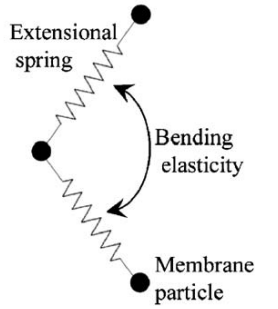
\includegraphics[width=0.3\linewidth]{mol3.png}
\caption{ Схема упругости при растяжении и изгибе между частицами в мембране \cite{hosseini:2009}.}
\label{fig:mpr}
\end{figure}

Для её описания используется четыре силы.
Первая сила возникает, когда стороны треугольников меняют свою длину.
$$\mathbf {F_I}=k_I(1- \frac{l}{l_0}) \mathbf {\tau}$$
где $l$--длина ребра, $l_0$--равновесная длина, $k_I$--коэфициент жёсткости, $\mathbf { \tau}$ --единичный вектор, направленный от одной вершины к другой.

К каждому узлу сходится несколько сторон, и каждая из них вносит свой вклад в общую силу F. Вторая сила определяется сжатием или расширением мембраны.  
$$\mathbf {p_s}=k_s(1- \frac{s}{s_0})$$
где $s$--площадь треугольника, $s_0$--площадь равновесного треугольника ,$k_s$--коэфициент расширения площади.

Третья сила пропорциональна изменению объема многогранника и прикладывается к вершинам треугольников в направлении, нормальном к поверхности. 
$$\mathbf {F_v}=k_v(1- \frac{v}{v_0}) s \mathbf{n}$$
где $v$ - объем многогранника, $v_0$ - равновесный объем, $k_v$ - коэффициент, $s$ - площадь
треугольного элемента, а $n$ - единичный нормальный вектор к этому треугольнику.

Четвёртая сила выражается через изгибающий момент\cite{hosseini:2009}.
$$\mathbf {M_i}=k_M \tan(\frac{\theta}{2})l \mathbf{\tau_i}$$
где $\theta$ - угол между соседними треугольными элементами, $k_m$ - коэффициент жесткости, $\mathbf{\tau_i}$- единичный вектор, сонаправленный с общим краем двух треугольников и $l$ - длина этой стороны.

Аналогичным образом могут быть смоделированы и другие клетки крови. Например, в отличие от эритроцитов, лейкоциты содержат ядро. Из-за этого они менее деформируемы, а их форма близка к сфере. Это влияет на их поведение в потоке крови.

Для определения параметров эритроцитов прибегают к методам численного моделирования~\cite{bessonov:2014}.

Фактически, можно легко указать на несколько недостатков данной модели. Например, рассмотрение всей клетки как однородной решетки делает невозможным учет любой органеллы в цитоплазме. Кроме того, эффективная упругость решетки зависит не только от пружинной постоянной, но и от конкретной формы, размера и топологии решетки. Это затрудняет сравнение между различными моделями и экспериментами. Более того, параметры модели на уровне частиц  модели не были систематически связаны с физиологическими измерениями; они должны принимать нереальные значения, чтобы предсказание было количественно сопоставимо с реальностью 


\subsection{Моделирование крови как неньютоновской жидкости}
Жидкость может считаться ньютоновской, если она удовлетворяет закону вязкости Ньютона, т.е. напряжение сдвига пропорционально скорости сдвига, а вязкость является константой пропорциональности, поэтому плазму крови, состоящую в основном из воды, можно считать ньютоновской. Однако у крови более сложные механические свойства. И мы предполагаем, что все макроскопические масштабы длины и времени достаточно велики по сравнению с масштабами длины и времени на уровне отдельного эритроцита. Таким образом, для упрощения построения модели и дальнейшей работы с ней можно рассматривать взвешенные клетки в плазме, как вязкую несжимаемую, неньютоновскую жидкость.\\

\textbf{Вязкость.}
Для начала рассмотрим простейшую конститутивную модель, основанную на предположении, что тензор дополнительных напряжений пропорционален
симметричной части градиента скорости.\\
$$\tau=2\mu (\dot{\gamma})D$$
где $\tau $-тензор дополнительных напряжений, $D=(\bigtriangledown u+\bigtriangledown u^T)$-тензор скорости деформации, $\mu (\dot{\gamma})$-скорость сдвига)
Зависимость $\mu (\dot{\gamma})$ находят разными способами. Например, в \cite{walburn:1976},   рассматривают зависимость вязкости от гематокрита и белка минусь-альбумин: \\
$\mu (\dot{\gamma})=K{\gamma}^{n-1},  K=C_1$ exp$(C_2 H_t).$\\
Полученные таким способом результаты вязкости оказались схожи с результатами, которые были получены в \cite{kim:2000} при помощи вязкозиметра.\\

\textbf{Вязкоупругость.}
Вязкоупругие жидкости — это вязкие жидкости, обладающие способностью накапливать и высвобождать энергию. Упругая энергия объясняется свойствами мембраны РНК, демонстрирующей релаксацию \cite{evans:1976} и зависящей от скорости сдвига.\\
Одной из простейших моделей, учитывающих вязкоупругость крови, является модель Максвелла \cite{thurston:1972}:\\
$\tau+\lambda_1(\delta\tau / \delta t)=2\mu D$,\\  где 
$\lambda_1$ 
- время релаксации, a 
$\delta\tau / \delta t$
- обобщение материальной производной по времени.
При построении данной модели полагают, что время релаксации зависит от скорости сдвига.
В \cite{thurston:1994} данный метод используют для понимания неньютоновского вязкого характера крови после устойоявшегося поток.

\textbf{Предел текучести.}
Предел текучести обычно рассматривается как постоянное материальное свойство жидкости. Но зафиксированные пределы текучести имели большой разброс, который, стоит отметить, зависел от множества факторов.
Поэтому предел текучести стоит рассматривать не как константу, а как функцию времени и связанную с тиксотропией, как было предложено в \cite{moller:2006}.
Более популярной моделью предела текучести является модель Кассона.
$$
\begin{aligned}
	&\sqrt{II_\tau} < \tau_Y\longrightarrow D=0 \\
	&\sqrt{II_\tau} > \tau_Y\longrightarrow
	\begin{cases}
		D   = \dfrac{1}{2\mu N}(1-\dfrac{\sqrt{\tau_Y}}{II_\tau})^2\tau \\[10pt]
		\tau= 2(\sqrt{\mu N}+\dfrac{\sqrt{\tau_Y}}{\sqrt[4]{4II_D}})^2
	\end{cases}
\end{aligned}
$$

В нашем случае предел текучести является параметра крови, например, для понимания, как будет вести себя кровь под влиянием какого-либо препарата, не станет ли она слишком вязкой или наоборот.
Однако, до сих пор использование предела текучести в качестве параметра моделирования крови остаётся спорным, в связи с неточностями его определения.

Данные методы применяется лишь в тех сосудах, где клетки достаточно малы и 
многочисленны, чтобы их отдельную индивидуальность можно было игнорировать, а их влияние на движение всей крови описывать усредненным способом. Так обстоит дело в крупных артериях (диаметр аорты, например, примерно в 2000 раз больше диаметра эритроцита). 
На практике эти методы применяются в изучении и моделировании сердечного выборса, печеночного кровотока, среднего артериального давления.

\subsection{Одномерные модели}

Привлекательность oдномерныx моделeй кровотока основана на разумных вычислительных затратах. Основные приложениями этих моделей являются транспорт газов крови и лекарств в организме, перераспределение кровотока при внешних или внутренних воздействиях, перераспределение кровотока в результате внутрисосудистых операций. Основными недостатками данных моделей являются сложность численных схем, высокая стоимость вычислений и спекулятивные граничные условия.Вычислительная область - это сосудистая одномерная сеть человека или ее части. Сеть может быть создана на основе общих анатомических данных, таких как справочник анатомических карт \cite{bunicheva:2013}, анатомические 3D модели или данные конкретного пациента.

В данном пункте мы осредняем все трёхмерные характеристики по поперечному сечению и рассматриваем одномерную задачу.

Обозначим через $t$ время, через $x$ - координату вдоль сосуда, через$A(t, x)$ - площадь поперечного сечения сосуда, $u(t, x)$ и $p$ - усредненную по сечению линейную скорость и трансмуральное давление крови. Баланс массы и импульса в переменных $(A, u, p)$ соответствует уравнениям

\begin{equation}
	\label{eq:mass-balance}
	\frac{\partial A}{\partial t}+\frac{\partial Au}{\partial x}=f_A,
\end{equation}
\begin{equation}
	\label{eq:momentum-balance}
	\frac{\partial u}{\partial t}+ \frac{\partial u^2/2+p/\rho}{\partial x}=f_u
\end{equation}

Правые части уравнений(масса источника или поглотителя на единицу длины, ускорение) зависят от моделируемого процесса. Эта модель была использована в \cite{bunicheva:2004} для моделирования воздействия гравитационной перегрузки на системное кровообращение. 

В одномерных моделях кровотока традиционное описание упругих свойств стенки сосуда обеспечивается отношением давления к площади поперечного сечения p(A). Прямой подход к получению отношения p(A) является точное одновременное измерение в естественных условиях давления и площади в разные моменты времени. Но, как можно понять, такой метод не всегда удобен в реальности.

Качественный анализ физических экспериментов подтверждает, что функция p(A) должна быть монотонной S-подобной кривой. Такая кривая удовлетворительно описывает  состояния как круглого, так и эллиптического сечения. На практике S-подобная  зависимость давления от площади часто аппроксимируется аналитической функцией. 

\begin{figure}[h]
\centering
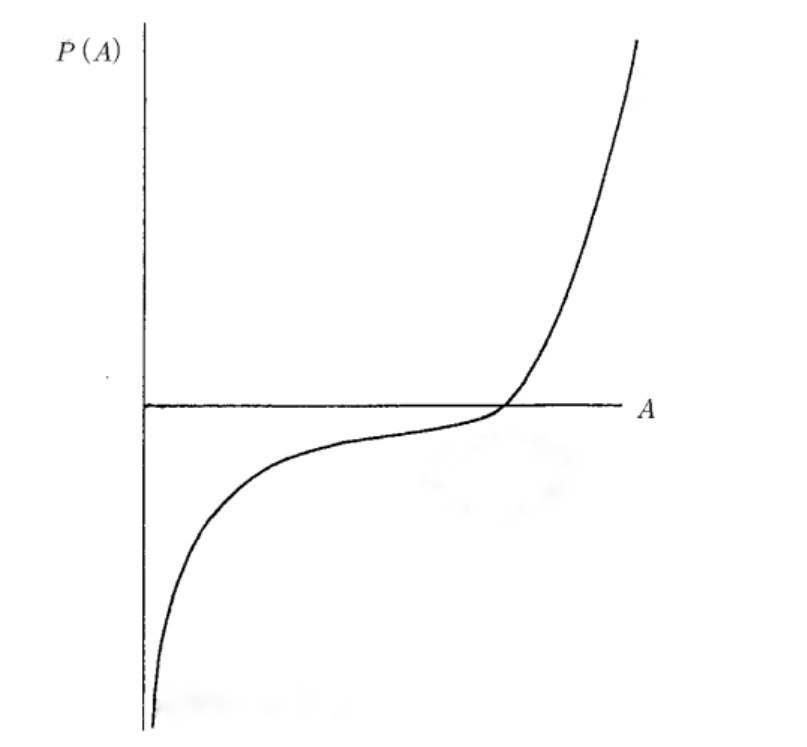
\includegraphics[width=0.3\linewidth]{IMG_20230309_021324_943-01.jpeg}
\caption{ График зависимости $P(A)$ \cite{pedly:1998}.}
\label{fig:mpr}
\end{figure}

Правильные упругие свойства артерий и вен могут быть описаны следующей функцией\cite{holodov:2001}:
\begin{equation}
	\label{eq:elast-prop}
	P(A)=\rho c^2_0 f(a/a_0), f(k)=\begin{cases}
        \exp(k-1)-1, k>1 \\ ln(k), k \leq 1
    \end{cases}
\end{equation}

Для каждого k-го сосуда известны законы сохранения массы и импульса(\ref{eq:conserv-mass}),(\ref{eq:conserv-mom}). И для замыкания системы уравнений необходимо учесть уравнение состояния описывающее изменение поперечного сечения сосуда в зависимости от трансмурального давления(\ref{eq:eq-state}).

\begin{equation}
	\label{eq:conserv-mass}
	\frac{\partial S_k}{ \partial t} + \frac{\partial(u_kS_k)}{\partial x}=\varphi _k(t,x,S_k,u_k,r_i)
\end{equation}

\begin{equation}
	\label{eq:conserv-mom}
	\frac{\partial u_k}{\partial t} + \frac{\partial(u_k^2/2+p_k/\rho_k)}{\partial x}= \psi_k(t,x,S_k,u_k,r_i)
\end{equation}

\begin{equation}
    \label{eq:eq-state}
    p_k(t,x)-p_*(t,x)=\rho_k c^2_{k0}f_k(S_k(t,x))
\end{equation}
где $t$— время, $x$— расстояние вдоль сосуда, $\rho$=const—плотность, $c_{k0}(t,x)$— скорость распространения малых возмущений,  $p_k(t,x)$- давление внутри сосуда(от атмосферного) $p_*(t,x)$— избыточное давление в тканях, окружающих сосуд, $S_ku_k=Q(t,x)$—кровоток, $\varphi _k(t,x,S_k,u_k,r_i)$-источник/утечка массы, $\psi_k(t,x,S_k,u_k,r_i)$—внечние силы(гравитация, трение и т.д.), $k=1,2,..$ —индекс сосуда.
\\ 
Другие обобщения модели эластичной стенки сосуда являются модели вязкоупругой стенки. В таких моделях зависимость $P(A)=F(A,\partial A / \partial t, \partial^2A / \partial t^2, \partial^2A / \partial x^2)$.\\

{Граничные условия}\\
Для одномерных моделей кровотока необходимы граничные условия на стыках сосудов, входах и выходах всети сосудов. Для всех сосудов граничные условия должны включать условия совместимости по характеристикам гиперболических уравнений(\ref{eq:mass-balance}), (\ref{eq:momentum-balance}).
В каждой конечной точке сосуда требуется только одно дополнительное условие совместимости.
Вторым условным граничным условием на стыке N сосудов является сохранение массы:
\begin{equation}
    \label{eq:mass-conserv}
    \sum_{k=k_1,k_2,...,k_N} \varepsilon_k A_k(t,x_k)u_k(t,x_k)=0
\end{equation}
где {$k_1,...,k_N$}-индексы сосудов, $\varepsilon_k=1, x_k=0$- для входящих сосудов,$\varepsilon_k=1, x_k=L_k$- для выходящих сосудов.

Другими граничными условиями является $N$ условий перепада давления:
\begin{equation}
    \label{eq:press-drop}
    p_k(A_k(t,x_k))-p^l(t)=\varepsilon_k R^l_k A_k(t,x_k)u_k(t,x_k)
\end{equation}

или $N$ интегральных условий сохранения Бернулли выражающих непрерывность полного давления:
\begin{equation}
    \label{eq:bernulli}
    u^2_k /2+p_k(A_k)/\rho=P^l
\end{equation}
где $p^l$ и $P^l$- давление и полное давление в точке с индексом 1, соответсвенно.

Подводя итог, можно сказать, что на каждом пересечении сосудов накладывается $2N + 1 $граничных условий в виде нелинейных алгебраических уравнений, которые могут быть 
эффективно сведены к $N + 1$ нелинейным уравнениям.

Выходы сети артерий и входы сети вен должны быть связаны с множеством мелких неучтенных сосудов, относящихся к микрососудистым регионам. Поток в таких сосудах не может быть описан одномерными моделями течения (\ref{eq:mass-balance})-(\ref{eq:conserv-mass}) из-за большого количества сосудов, сложной структуры микрососудистых сетей и неньютоновской реологии крови.

Более простой подход заключается в том, чтобы объединить артерий и вены в точки соединения, где выполняются (\ref{eq:mass-conserv}),(\ref{eq:press-drop}). Коэффициенты сопротивления $ R^l_k$ оцениваются  по известному перепаду давления между артериями и венами. Чем больше сосудистая сеть, тем меньше сосудов объединяются, тем выше точность метода. Более подходящие граничные условия оттока: отдельные участки мелких артерий и микроциркуляции моделируются как структурированные деревья, чей импеданс корней может быть оценен из линеаризации управляющих уравнений.

Многие авторы \cite{alastruey:2008} выполняют сопряжение во временной области 1D моделей кровотока с электрическими цепями (единичными параметрами) 0D моделей. 0D модели обеспечивают корректные граничные условия для глобальных моделей кровотока.
\\
Численные схемы

С математической точки зрения, одномерная модель кровотока представляет собой алгебраическо-дифференциальную систему, состоящую из набора гиперболических уравнений в сосудах и набора алгебраических уравнений на стыках и входах/выходах сети сосудов. Дробные временные шаги неявно-явных схем разделяют вычисления на отдельные локализованные части и поэтому легко распараллеливаются.

Мы рассматриваем системный круг, представленный двумя связанными сетями артерий и вен(рис.5). Сосудистая система состоит из 341 сосуда с анатомически адекватными свойствами (длина, диаметр, упругие свойства), вен и артерий. Вены и артерии соединены в 162 точках, на которые наложены граничные условия (\ref{eq:mass-conserv}),(\ref{eq:press-drop}). 

\begin{figure}[h]
\centering
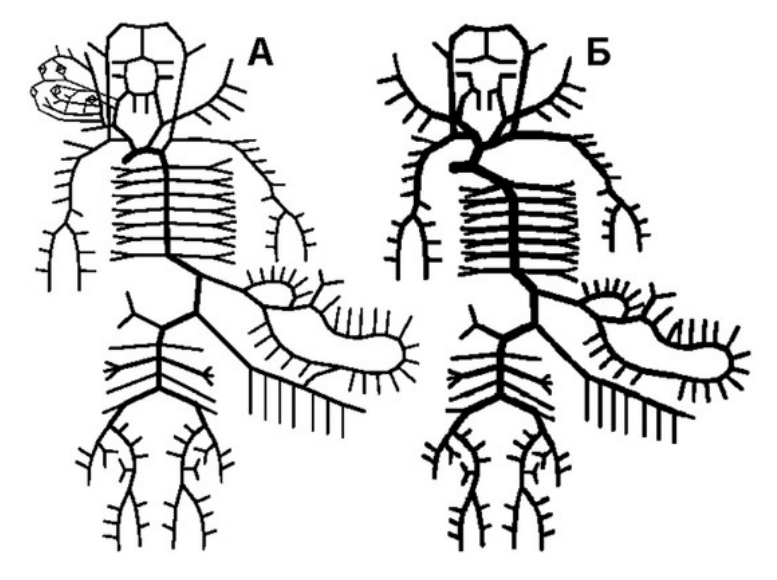
\includegraphics[width=0.5\linewidth]{krug.png}
\caption{Упрощённая структура сосудов системного круга. А—артерии, Б—вены.}
\label{fig:mpr}
\end{figure}

В каждом сосуде мы вводим одномерную равномерную сетку и дискретизируем систему (\ref{eq:mass-balance}),(\ref{eq:momentum-balance}) методом монотонных характеристик первого порядка. Уравнения расширяются набором жестких ОДЕ, которые описывают работу сердца в терминах усредненной по объему модели.

Система жестких ОДУ, решаемая неявным методом Рунге-Кутта третьего порядка, обеспечивает граничные условия на входе и выходе сердца. Алгебраическая дифференциальная система (\ref{eq:mass-balance}), (\ref{eq:momentum-balance}), (\ref{eq:mass-conserv}),(\ref{eq:press-drop}) в сочетании с зависимостью давления от площади и соответствующими граничными условиями на входе и выходе сердца и микроциркуляторных областях, решается по схеме с дробным шагом по времени схема, которая разделяет вычисления на локальные независимые части (отдельные сосуды и отдельные точки соединения).

На гиперболическом подэтапе мы применяем явный метод характеристик для каждого сосуда и контролируем шаг по времени с помощью ограничения устойчивости $\tau = 0.9 s_{max}$, где $s_{max}=max_{k,i}|\lambda _{k,i}|/h_k$, где $h_k$ - размер сетки в сосуде $k$, $\lambda$ - размер сетки в сосуде $k$,  $\lambda _{k,i}$ - наибольшее (по величине) собственное значение якобиана для  (\ref{eq:mass-balance}), (\ref{eq:momentum-balance}) в точке сетки.

В алгебраическом подэтапе мы применяем метод Ньютона для системы уравнений в каждом узле пересечения. Система состоит из уравнений (\ref{eq:mass-conserv}),(\ref{eq:press-drop}) и условие совместимости по характеристикам  (\ref{eq:mass-balance}), (\ref{eq:momentum-balance}). Влияние атеросклеротической бляшки учитывается в модели эластичной стенки. Здоровые сосуды описываются уравнением (\ref{eq:elast-prop}), обеспечивающим достоверную корреляцию с экспериментальными кривыми. Атеросклеротические артерии рассматриваются как трехслойные цилиндрические оболочки, деформированные внутренним давлением крови. Внутренний и внешний слои оболочки - это фиброзная крышка и стенка артерии, соответственно. Деформации фиброзной пробки и стенки сосуда моделируются с помощью волоконно-эластичной модели. В простейшей версии волоконной осесимметричной модели оболочка представлена набором кольцевых волокон, которые сопротивляются только растяжению и сжатию волокон, как неогуковские материалы.

\begin{equation}
    \label{eq:force-density}
    \mathbf{F}=\frac{\partial}{\partial s}(T\mathbf{\tau}), T=\mu(|\frac{\partial \mathbf{X}}{\partial s}|^2-|\frac{\partial \mathbf{X}}{\partial s}|^{-2}).
\end{equation}

Здесь $\mathbf{F}$ обозначает плотность локальной силы, $T(s)$ обозначает натяжение волокна, $\tau =\partial X/\partial s^{-1}$ единичный касательный вектор, $X(s)$ представляет собой положение точек волокна в пространстве, координата Лагранжа s - длина дуги волокна в ненапряженном состоянии. Липидный пул (промежуточная оболочка) имитируется набором радиальных пружин с нелинейной зависимостью между силой реакции и смещением

Отношение давления к площади атеросклеротической артерии получено из предположения о статическом равновесии стенки: внутреннее давление крови уравновешивается упругими силами вышеупомянутой системы волоконных пружин, возникающими при ее смещении. На основе смещений можно рассчитать поперечную площадь сечения $A$ как реакцию на любое давление крови. 
Восстановление равновесного состояния получено в рамках его численной аппроксимации: конечно-разностная дискретизация (\ref{eq:force-density}) приводит к системе нелинейных алгебраических уравнений, которая должна быть решена итерационно методом Ньютона.

Численная модель "волокно-пружина" имеет преимущества прямые обобщения с другими 
типами волокон и, таким образом, может быть распространена на гораздо более широкий 
класс геометрий бляшек.

\begin{figure}[h]
\centering
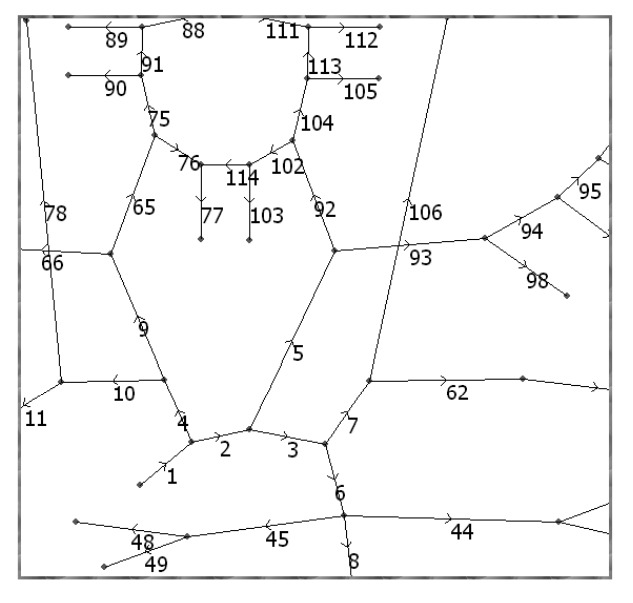
\includegraphics[width=0.4\linewidth]{chast.png}
\caption{Участок сосудов системного круга.}
\label{fig:mpr}
\end{figure}

В эксперименте мы предполагаем, что левая общая сонная артерия (№5 на рис.6) 
повреждена протяженной атеросклеротической бляшкой с просветом 10\%, 30\%, 50\% и 
100\%. Коэффициенты упругой бляшки взяты из \cite{vassilevski:2011}. Профили скоростей в наружном 
сонном продолжении (№94) и артериях круга Уиллиса (№104,102) показаны на рис.7. 
Наиболее заметные изменения в скорости происходят в случае бляшек с просветом 30\% и 
10\%. В малой артерии Виллисова круга (104) и на продолжении левой наружной сонной 
артерии (94) наблюдается значительное снижение скорости крови.

\begin{figure}[h]
\centering
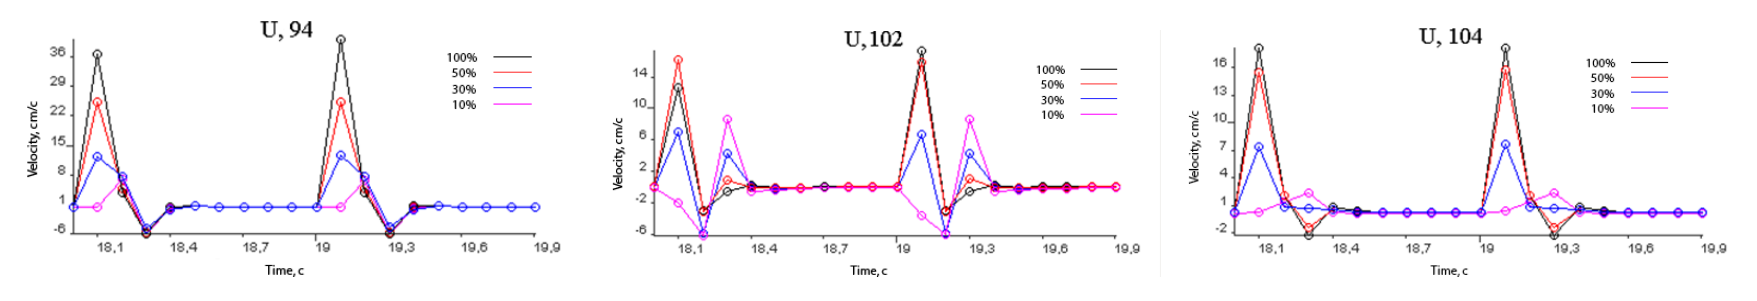
\includegraphics[width=0.9\linewidth]{grap.png}
\caption{Скорость (см/с) в сосудах 94, 102, 104 для различных просветов. Здоровый сосуд
соответствует 100\% просвету}
\label{fig:mpr}
\end{figure}0


\newpage
\addcontentsline{toc}{section}{Список используемой литературы}
\begin{thebibliography}{}
    \bibitem{litlink1}  Boileau E. et al A benchmark study of numerical schemes for one-dimensional arterial blood flow modelling // Int. J. Numer. Meth. Biomed. Engng. 2015.
    \bibitem{litlink2} F. J. Walburn, D. J. Schneck. A constitutive equation for whole human blood. Biorheology, 13 (1976), 201–210.
    \bibitem{litlink3} S. Kim, Y.I . Cho, A. H. Jeon, B. Hogenauer, K. R. Kensey. A new method for blood viscosity measurement. J. Non-Newtonian Fluid Mech., 94 (2000), 47-56.
    \bibitem{litlink4}  E. A. Evans, R. M. Hochmuth. Membrane viscoelasticity. Biophys. J., 16 (1976), no. 1, 111.
    \bibitem{litlink5} G. B. Thurston. Viscoelasticity of human blood. Biophys. J., 12 (1972), 1205–1217.
    \bibitem{litlink6} G.B. Thurston. Non-Newtonian viscosity of human blood: Flow induced changes in microstructure. Biorheology, 31 (1994), no. 2, 179–192.
    \bibitem{litlink7} P.C. F. Moller, J. Mewis, D. Bonn. Yield stress and thixotropy: on the difficulty of measuring yield stress in practice. Soft Matter, 2 (2006), 274–288.
     \bibitem{litlink8} P.C. F. Moller, J. Mewis, D. Bonn. Yield stress and thixotropy: on the difficulty of measuring yield stress in practice. Soft Matter, 2 (2006), 274–288.
    \bibitem{litlink9}  S.M. Hosseini, J.J. Feng. A particle-based model for the transport of erythrocytes in capillaries. Chem. Eng. Sci., 64 (2009), 4488-4497.
    \bibitem{litlink10} N. Bessonov, E. Babushkina, S.F. Golovashchenko, A. Tosenberger, F. Ataullakhanov, M. Panteleev, A. Tokarev, V. Volpert. Numerical modelling of cell distribution in blood flow. Math. Model. Nat. Phenom., 9 (2014), no. 6, 69-84.
    \bibitem{litlink11} A. Ya. Bunicheva, M. A. Menyailova, S. I. Mukhin, N. V. Sosnin, A. P. Favorskii. Studying the influence of gravitational overloads on the parameters of blood flow in vessels of greater circulation. Mathematical Models and Computer Simulations, 5 (2013), no. 1, 81-91.
    \bibitem{litlink12} A.Ya. Bunicheva, S.I. Mukhin, N.V. Sosnin, A.P. Favorskii. Numerical experiment in hemodynamics. Differential Equations, 40 (2004), no. 7, 984-999.
    \bibitem{litlink13} A.S. Kholodov. Some dynamical models of external breathing and haemodynamics accounting for their coupling and substance transport. Computer Models and Medicine Progress, Nauka, Moscow, 127-163, 2001.
    \bibitem{litlink14} Blausen.com staff. “Blausen gallery 2014”. Wikiversity Journal of Medicine. DOI:10.15347/wjm/2014.010
    \bibitem{litlink15} T.J. Pedley, X.Y. Luo. Modelling flow and oscillations in collapsible tubes. Theoretical and Computational Fluid Dynamics, 10 (1998), 277-294.
    \bibitem{litlink16} S.S. Grigorjan, Y.Z. Saakjan, A.K. Tsatutjan. To the theory of Korotkoff method. Biomechanics, (1984), no. 15-16,54-75.
    \bibitem{litlink17}J. Alastruey, K.H. Parker, J. Peir´o, S.J. Sherwin. Lumped parameter outflow models for 1-D blood flow simulations: effect on pulse waves and parameter estimation. Communications in Computational Physics, 4 (2008), no. 2, 317-336.
    \bibitem{litlink18} Y. Vassilevski, S. Simakov, V. Salamatova, Y. Ivanov, T. Dobroserdova. Vessel wall models for simulation ofatherosclerotic vascular networks. Math. Model. Nat. Phenom., 6 (2011), no. 7, 82-99
    \bibitem{litlink19} https://app.rlsnet.ru/api/storage/books/jpg/253_P1_05_02_e
    
    \bibitem{litlink20} J.A.G. Rhodin  Architecture of the vessel wall / The Handbook of Physiology. The Cardiovascular System. Bethesda, Maryland. 1980. T. 2. С. 1–31.
    
\end{thebibliography}






\end{document}